\documentclass[a4paper,10pt]{article}

% \usepackage{amsmath}
% \usepackage{amssymb}
% \usepackage{amsfonts}
% \usepackage{amsmath}
% \usepackage{graphicx}
% \usepackage{tabularx}

\usepackage{amssymb}
\usepackage{epsfig,psfrag}
\usepackage[german,american]{babel}
\usepackage{amsmath}
%\usepackage{refcheck}
\usepackage{epstopdf}
\usepackage{color}
\usepackage{tabularx}
\usepackage{siunitx}
\usepackage{url}


% \usepackage{graphicx}
% \usepackage{subcaption}
% \usepackage{appendix}
% \usepackage[german,american]{babel}
% \usepackage{amsmath}
% \usepackage{amssymb}
% \usepackage{url}
% %\usepackage{refcheck}
% \usepackage{rotating}

\title{Optimization of District Heating Networks}
\author{Florian M\"uller}
\date{January, 2015}

\begin{document}

\maketitle

This is a report on the results of Florian M\"uller's employment from October 2014 until December 2014 as a research assistant in the field of optimization of district heating networks at SuAT/ETH Z\"urich. 
Florian M\"uller collaborated with Jimeno Fonseca.

\tableofcontents

\section{The District Heating Optimization Problem}

A centralized pumping and heating plant of a district must provide hot water to all buildings within its district through a network of pipes in order to meat the heating demands of the buildings. 

The pipe network consists of a supply and return network rooted at the plant. 
The supply network transports hot water to all the buildings. 
After the heat is extracted, the cold water is transported back to the plant through a return network.
This yields a hydraulically closed thermo-hydraulic network driven by the pumping and heating of the plant.  

Each building must be supplied with a specific volume flow of water at a minimum inflow pressure and minimum inflow temperature. 
Within each building, the water is then expanded over a heat exchanger resulting in a pressure and temperature drop.

The network layout is restricted to the roads within the district.

For each edge within the network, different types of pipes corresponding to a discrete range of diameters are available. 
The choices of pipe types of the different edges influence the investment cost of the network. 
Moreover, the choices of pipe types influence the pressure losses and heat losses of the network and therefore the pumping and heating of the plant and the associated operation cost.

In summary, we seek a supply and return network of pipes complying with the district's roads and connecting the plant with all the buildings of the district. 
The pumping and heating of the plant must be such that the building's volume flow, inflow pressure and inflow temperature requirements are met. 
Sometimes, an additional minimum pipe network reliability requirement is formulated, see for example~\cite{Afshar}. 
The district heating optimization problem can then be stated as follows. 
Subject to all these constraints, choose the pipe types and the pumping and heating of the plant such that the operation cost of the plant and the investment cost of the pipe network are minimal.



\section{Context}

We divide the district heating optimization problem into different parts, namely:
\begin{itemize}
  \item Layout problem: the problem of specifying the edges, i.e. how the plant and the different building nodes are connected.
  This does not include the specification of pipe types.
  \item Hydraulic problem: the problem of specifying the pipe types of the different edges and the pumping of the plant.
  \item Thermal problem: the problem of specifying the heating of the plant.
\end{itemize}
In order to rigorously solve the district heating optimization problem one needs to simultaneously consider all three subproblems, one has to find a corresponding mixed integer convex formulation and one needs to be able to numerically solve this program within reasonable time. 
Currently, this is clearly out of reach for us.

In the following, we divide the relevant literature into two types of approaches. 

\subsection{First Approach}
The first type of approach tackles the district heating optimization problem or rather subproblems of it with heuristic optimization techniques such as simulated annealing or genetic algorithm. 
These approaches do not rely on a convex formulation of the problem and can therefore not guarantee that their solutions are globally optimal.
Examples of the first type of approach are:
\begin{itemize}
  \item \cite{Cunha}: A simulated annealing approach is deployed for the hydraulic problem.
  \item \cite{Djebedjian}: A genetic algorithm approach is deployed for the hydraulic problem.
  \item \cite{Afshar}: A genetic algorithm approach is used for the simultaneous solution of the layout and hydraulic problems while imposing a pipe network reliability constraint.
\end{itemize}

\subsection{Second Approach}
The second type of approach uses mixed integer and mostly linear or non-linear convex programming. 
Examples of the second type of approach are:
\begin{itemize}
  \item \cite{Hendrickson}: A non-linear convex formulation for the hydraulic problem is provided.
  \item \cite{Bragalli}: A mixed integer solver is applied to a mixed integer non-convex formulation of the hydraulic problem. 
  Due to the lack of convexity, the solution is not guaranteed to be globally optimal.
  \item \cite{Raghunathan}: The hydraulic problem is formulated in terms of a mixed integer non-linear convex program. 
  The program is then solved with a linearization based branch and cut algorithm with tailored cuts.
\end{itemize}

\subsection{Our Approach}
Our approach belongs to the second type. More specifically:

\subsubsection{Hydraulic Problem}
\begin{itemize}
  \item We consider the hydraulic problem subject to the following assumptions:
  \begin{itemize}
    \item The pipe network layout is predefined.
    \item The flow directions within the pipe network are predefined. 
  \end{itemize}
  Hence, the hydraulic problem is the problem of specifying the pipe types of the different edges and the pumping of the plant.
  \item We approximate the pressure drop functions of the hydraulic problem with linear cuts.
  \item We solve the hydraulic problem based on a mixed integer linear program inspired by~\cite{Hendrickson} and~\cite{Raghunathan}. 
  \item We use Matlab's \texttt{intlinprog} to solve the hydraulic mixed integer linear program. 
  Due to linearity, a globally optimal solution for the (isolated and linearized) hydraulic problem is guaranteed.
\end{itemize}
\subsubsection{Reduced Hydraulic Problem}
\begin{itemize}
  \item For practical reasons, we also consider a reduced version of the hydraulic problem subject to the following assumption:
  \begin{itemize}
    \item In contrast to the hydraulic problem, the pipe types of the different edges are predefined.
  \end{itemize}
  Hence, the reduced hydraulic problem is the problem of specifying the pumping of the plant only.
  \item We approximate the pressure drop functions of the reduced hydraulic problem with linear cuts.
  \item We solve the reduced hydraulic problem based on a linear program.
  \item We use Matlab's \texttt{linprog} to solve the reduced hydraulic linear program.
  Due to linearity, a globally optimal solution for the (isolated and linearized) reduced hydraulic problem is guaranteed.
\end{itemize}
\subsubsection{Thermal Problem}
\begin{itemize}
  \item We consider the thermal problem subject to the following assumption:
  \begin{itemize}
    \item The volume flows of the different edges are predefined.
  \end{itemize}
  Hence, the thermal problem is the problem of specifying the heating of the plant only.
  \item We solve the thermal problem based on a linear program.
  \item We use Matlab's \texttt{linprog} to solve the thermal linear program.
  Due to linearity, a globally optimal solution for the (isolated) thermal problem is guaranteed.
\end{itemize}
\subsubsection{Additional Remarks}
\begin{itemize}
  \item One hack to approach the layout and hydraulic problem simultaneously is to add a virtual pipe type to the set of available pipe types. 
  If this virtual pipe type has zero diameter and zero investment cost and if the pipe network layout covers all the roads of the district, we have integrated the layout and the hydraulic problem. 
  However, the virtual pipe type approach leads us to numerical problems and is therefore not further investigated.
  \item Predefining the flow directions is a restriction in looped networks. 
  Furthermore, it is in contrast to~\cite{Raghunathan} where flow directions are not predefined. 
  Because in our case, non-predefined flow directions imply more additional variables than in~\cite{Raghunathan}\footnote{This is because in contrast to~\cite{Raghunathan}, we have to comply with a minimum volume flow for the different pipe types.} and because we do not work with a dedicated mixed integer solver, we can computationally not afford to not predefine the flow directions.
  \item Our set of pipe types includes twin pipes only. 
  With this, we always have identical pipes for the supply and return network. 
  Moreover, we enforce hydraulic symmetry meaning that the hydraulic conditions in terms of volume flow and pressure of the supply and return network are just inversions of each other. 
  However, this does not hold for the thermal conditions.
  \item Apart from Matlab implementations based on \texttt{intlinprog} and \texttt{linprog}, we provide Python wrapper implementations such that Matlab's \texttt{intlinprog} and \texttt{linprog} can be called from Python.
  \footnote{Matlab and Python use one-based and zero-based indexing, respectively. 
  In the remainder of this report, we assume one-based indexing.}
\end{itemize}



\section{Layout Problem}

We assume that the layout problem is already solved. 
Its solution is given in terms of nodes and edges for the supply and return network. 
Furthermore, the flow directions of the supply and return network are predefined.

\subsection{Data}\label{sec:layoutData}
%The layout data describes the layout of the supply network.

\begin{tabularx}{\textwidth}{llX}
  $\mathcal{N}$ &[-]& $\mathcal{N} = \{1,2,\dots,N\}$,
                      set of all node indices $n$\\
  $\mathcal{E}$ &[-]& $\mathcal{E} = \{1,2,\dots,E\}$,
                      set of all edge indices $e$\\
  $s_e^{spp}$         &[-]& supply edge $s_e^{spp}=[n,n']$, 
                      indicating a flow from node $n$ to $n'$\\
  $s_e^{rtn}$         &[-]& return edge $s_e^{rtn}=[n',n]$, 
                      indicating a flow from node $n'$ to $n$,
                      if $s_e^{spp}=[n,n']$, then $s_e^{rtn}=[n',n]$ (in order to agree with hydraulic symmetry)\\
  $n^{pl}$      &[-]& plant node index
\end{tabularx}



\section{Hydraulic Problem}

Here, we formulate a mixed integer linear program for solving the hydraulic problem assuming that the layout data of section~\ref{sec:layoutData} is given.
Because we assume hydraulic symmetry, it is sufficient to consider the supply network only. 

\subsection{Data}\label{sec:hydraulicData}

The hydraulic data consists of the layout data of section~\ref{sec:layoutData}.
Additionally, we define the following hydraulic data.

\begin{tabularx}{\textwidth}{llX}
  $\rho$ &[\si{kg.m^{-3}}]& density of water\\
  $\nu$ &[\si{m^{2}.s^{-1}}]& kinematic viscosity of water\\
  $\eta^{pump}$ &[-]& plant pump efficiency\\
  $c^{pump}$ &[\si{CHF.W^{-1}.y^{-1}}]& plant pump operation cost factor, 
                                        annualized\\
  $p_n^{rq}$ &[\si{pa}]& requested pressure of node $n$,
                         if supply pressure above $p_n^{rq}$ at a building node, then the resulting exceed pressure is released by an expansion over a valve
                         \footnote{Even though we might waist a lot of exceed pressure here, it seems to be the only practical approach in connection with twin pipes.
                         Together with the fact that we allow for twin pipes only, this approach ensures hydraulic symmetry.
                         Hydraulic symmetry with respect to zero pressure implies that the internal pressure drop over a building at node $n$ is $2 p_n^{rq}$ (excluding the exceed pressure).}\\
  $\dot{v}_n^{rq}$ &[\si{m^{3}.s^{-1}}]& requested volume flow of node $n$,
                                         ignored for plant node,
                                         negative for the building nodes,
                                         zero for other nodes\\
  $\dot{v}^{pl}$ &[\si{m^{3}.s^{-1}}]& volume flow of plant,                                      
                                       should fulfill $\dot{v}^{pl}=-\sum_{n\in\mathcal{N}\setminus n^{pl}}\dot{v}_n^{rq}$\\
  $L_e$ &[\si{m}]& lengths of edge $e$\\
  $\mathcal{I}$&[-]& $\mathcal{I} = \{1,2,\dots,I\}$,
                   set of all pipe type indices $i$\\
  $d_i$ &[\si{m}]& pipe diameter of pipe type $i$\\
  $c_i$ &[\si{CHF.m^{-1}.y^{-1}}]& pipe investment cost factor of pipe type $i$,
				    annualized\\
  $r_i$ &[\si{m}]& pipe roughness of pipe type $i$\\
  $\dot{v}_i^{min}$ &[\si{m^{3}.s^{-1}}]& minimally allowed volume flow of pipe type $i$\\
  $\dot{v}_i^{max}$ &[\si{m^{3}.s^{-1}}]& maximally allowed volume flow of pipe type $i$\\
  $\phi_i$ &[\si{pa.m^{-1}}]& pressure drop function of pipe type $i$,
	                      relating volume flow to pressure drop per length\\
  $\mathcal{K}$&[-]& $\mathcal{K} = \{1,2,\dots,K\}$,
                     set of all linear cut indices $k$\\
  $a_{k,i}$ &[\si{pa.s.m^{-4}}]& first linear cut coefficient of linear cut $k$ and pipe type $i$\\
  $b_{k,i}$ &[\si{pa.m^{-1}}]& second linear cut coefficient of linear cut $k$ and pipe type $i$

\end{tabularx}

\subsection{Variables}\label{sec:hydraulicVariables}

\begin{tabularx}{\textwidth}{llX}
  $x_{i,e}$ &[-]& decision binary variable of pipe type $i$ and edge $e$,
  if $x_{i,e}=1$, then pipe type $i$ is chosen for edge $e$,
  if $x_{i,e}=0$, then pipe type $i$ is not chosen for edge $e$\\
  $\dot{v}_{i,e}$ &[\si{m^{3}.s^{-1}}]& volume flow disjunction variable of pipe type $i$ and edge $e$,
  if $x_{i,e}=1$, then $\dot{v}_{i,e}$ equals the volume flow of edge $e$,
  if $x_{i,e}=0$, then $\dot{v}_{i,e}=0$\\
  $p_n$ &[\si{pa}]& pressure of node $n$
\end{tabularx}

\subsection{Pressure Drop}
The pressure drop function of pipe type $i$ relates volume flow $\dot{v}$ to pressure drop per length $\Delta p/L$.
It is based on the Darcy-Weisbach equation~\cite{DarcyWeisbach},
$$\frac{\Delta p}{L}=\phi_i(\dot{v})=\frac{8 f^{Darcy}\rho}{\pi^2 d_i^3}\dot{v}^2,$$
where the Darcy friction factor is approximated with the Swamee-Jain equation~\cite{SwameeJain},
$$f^{Darcy}=0.25\left[\log_{10}\left(\frac{r_i}{3.7 d_i}+5.74 Re^{-0.9}\right)\right]^{-2},$$
and where the Reynolds number reads,
$$Re=\frac{4\dot{v}}{\pi \nu d_i}.$$
Strictly speaking, the Swamee-Jain equation is only valid for fully turbulent flow with $Re>4000$.
This restriction should be enforced through an appropriate choice of $\dot{v}_i^{min}$.
Another issue is that the Swamee-Jain equation has a singularity at $r_i/(3.7 d_i)+5.74 Re^{-0.9}=1$ and the resulting $\phi_i(\dot{v})$ is therefore only conditionally convex.
However, this issue is resolved through the linearization procedure of section~\ref{sec:lin} below.

\subsection{Linearized Pressure Drop}\label{sec:lin}

We assume that $\phi_i(\dot{v})$ is non-linear convex under the condition that $\dot{v}_i^{min}\le\dot{v}\le\dot{v}_i^{max}$. 
We approximate the conditionally non-linear convex $\phi_i(\dot{v})$ by a set of linear cuts. 
For all $k\in\mathcal{K}$, we define the volume flow linearization point $k$ of pipe type $i$ as,
$$\dot{v}_{k,i}^{lin} = \dot{v}_i^{min}+\frac{\dot{v}_i^{max}-\dot{v}_i^{min}}{K-1}(k-1).$$
We further define the linear cuts as,
$$a_{k,i}\dot{v}+b_{k,i},$$
with,
$$a_{k,i}=\frac{d \phi_i}{d \dot{v}}(\dot{v}=\dot{v}_{k,i}^{lin}),$$
and,
$$a_{k,i}\dot{v}_{k,i}^{lin}+b_{k,i}=\phi_i(\dot{v}_{k,i}^{lin}).$$
For illustration, we plot $\phi_i(\dot{v})$ and the linear cuts $a_{k,i}\dot{v}+b_{k,i}$ $\forall k\in\mathcal{K}$ and for fixed $i$.
See figure~\ref{fig:1}.

\begin{figure}
  \centering
  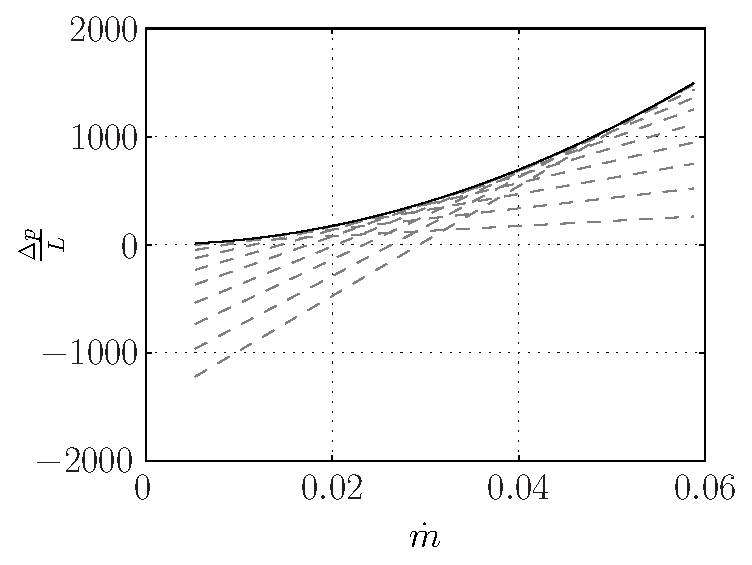
\includegraphics[width=.6\textwidth]{Fig/cuts}
  \caption{$k\in\mathcal{K}$, fixed $i$; black solid line: $\frac{\Delta p}{L}=\phi_i(\dot{v})$; gray dashed lines: $\frac{\Delta p}{L}=a_{k,i}\dot{v}+b_{k,i}$}\label{fig:1}
\end{figure}

\subsection{Mixed Integer Linear Program}

Here, we formulate the mixed integer linear program for the solution of the hydraulic problem.

The objective function consisting of annualized pump operation and annualized pipe investment cost reads,
\begin{align}
2 p_{n^{pl}} \dot{v}^{pl}\frac{c^{pump}}{\eta^{pump}} + \sum_{e\in\mathcal{E}}\sum_{i\in\mathcal{I}} x_{i,e} L_e c_i.
\end{align}
The factor $2 p_{n^{pl}}$ represents the pressure drop over the supply network and over the return network.

The integral constraints read,
\begin{align}
 x_{i,e} &\in \mathcal{Z} &\forall& i\in\mathcal{I},e\in\mathcal{E}&,
\end{align}
where $\mathcal{Z}$ denotes the set of all integers.

The upper and lower bounds read,
\begin{align}
 0&\le x_{i,e}\le1  &\forall& i\in\mathcal{I},e\in\mathcal{E} &,\\
 p_n^{rq}&\le p_{n} &\forall& n\in\mathcal{N}   &.
\end{align}

The inequality constraints read,
\begin{align}
 \dot{v}_{i,e}&\ge x_{i,e}\dot{v}_i^{min}&\forall& i\in\mathcal{I},e\in\mathcal{E} &,\\
 \dot{v}_{i,e}&\le x_{i,e}\dot{v}_i^{max}&\forall& i\in\mathcal{I},e\in\mathcal{E} &,\\
 \sum_{i\in\mathcal{I}} a_{k,i}\dot{v}_{i,e} +b_{k,i}x_{i,e} &\le \frac{p_{n}-p_{n'}}{L_e}&\forall& e\in\mathcal{E},k\in\mathcal{K}&,
\end{align}
where $s_e^{spp}=[n,n']$.

The equality constraints read,
\begin{align}
 \sum_{i\in\mathcal{I}} x_{i,e}&=1&\forall& e\in\mathcal{E} &,\\
 \sum_{e\in \mathcal{E}^+} \sum_{i\in\mathcal{I}} \dot{v}_{i,e} - \sum_{e\in \mathcal{E}^-} \sum_{i\in\mathcal{I}} \dot{v}_{i,e} + \dot{v}_n^{rq} &= 0&\forall& n\in\mathcal{N}\setminus n^{pl} &.
\end{align}
Here, $\mathcal{E}^+$ denotes the set of all edge indices $e$ for supply edges $s_e^{spp}=[n',n]$ incident on node $n$.
Furthermore, $\mathcal{E}^-$ denotes the set of all edge indices $e$ for supply edges $s_e^{spp}=[n,n']$ outcident from node $n$.



\section{Reduced Hydraulic Problem}

Here, we formulate a linear program for solving the reduced hydraulic problem assuming that pipe types of the different edges are predefined in terms of given $x_{i,e}$ of section~\ref{sec:hydraulicVariables}.
Again, due to the hydraulic symmetry assumption, it is sufficient to consider the supply network only.

\subsection{Data}

The reduced hydraulic data consists of the hydraulic data of section~\ref{sec:hydraulicData} and the hydraulic variables of section~\ref{sec:hydraulicVariables}.
Additionally, we define the following reduced hydraulic data.

\begin{tabularx}{\textwidth}{llX}
  $i_e$ &[-]& decision pipe type variable of edge $e$,
              indicating the pipe type chosen for edge $e$,
              derived from $i_e=\texttt{find}_{i\in\mathcal{I}}(x_{i,e}==1)$\ \ \footnote{This expression is pseudo Matlab syntax.},
              with $x_{i,e}$ of section~\ref{sec:hydraulicVariables}\\
  $\dot{v}_e^{min}$ &[\si{m^{3}.s^{-1}}]& minimally allowed volume flow of edge $e$,
                                          derived from $\dot{v}_e^{min}=\dot{v}_{i=i_e}^{min}$,
                                          with $\dot{v}_i^{min}$ of section~\ref{sec:hydraulicData}\\
  $\dot{v}_e^{max}$ &[\si{m^{3}.s^{-1}}]& maximally allowed volume flow of edge $e$,
                                          derived from $\dot{v}_e^{max}=\dot{v}_{i=i_e}^{max}$,
                                          with $\dot{v}_i^{max}$ of section~\ref{sec:hydraulicData}\\
  $a_{k,e}$ &[\si{pa.s.m^{-4}}]& first linear cut coefficient of linear cut $k$ and edge $e$,
                                 derived from $a_{k,e}=a_{k,i=i_e}$,
                                 with $a_{k,i}$ of section~\ref{sec:hydraulicData}\\
  $b_{k,e}$ &[\si{pa.m^{-1}}]& second linear cut coefficient of linear cut $k$ and edge $e$,
                               derived from $b_{k,e}=b_{k,i=i_e}$,
                               with $b_{k,i}$ of section~\ref{sec:hydraulicData}
\end{tabularx}

\subsection{Variables}\label{sec:reducedHydraulicVariables}

\begin{tabularx}{\textwidth}{llX}
  $\dot{v}_{e}$ &[\si{m^{3}.s^{-1}}]& volume flow of edge $e$\\
  $p_n$ &[\si{pa}]& pressure of node $n$
\end{tabularx}

\subsection{Linear Program}

Here, we formulate the linear program for the solution of the reduced hydraulic problem.

The objective function consisting of annualized pump operation cost reads,
\begin{align}
2 p_{n^{pl}} \dot{v}^{pl}\frac{c^{pump}}{\eta^{pump}}.
\end{align}
The factor $2 p_{n^{pl}}$ represents the pressure drop over the supply network and over the return network.

The lower and upper bounds read,
\begin{align}
 p_n^{rq}   &\le p_{n}          &\forall& n\in\mathcal{N} &,\\
 \dot{v}_{e}&\ge \dot{v}_e^{min}&\forall& e\in\mathcal{E} &,\\
 \dot{v}_{e}&\le \dot{v}_e^{max}&\forall& e\in\mathcal{E} &.
\end{align}

The inequality constraints read,
\begin{align}
 a_{k,e}\dot{v}_{e} +b_{k,e} &\le \frac{p_{n}-p_{n'}}{L_e}&\forall& e\in\mathcal{E},k\in\mathcal{K}&,
\end{align}
where $s_e^{spp}=[n,n']$.

The equality constraints read,
\begin{align}
 \sum_{e\in \mathcal{E}^+} \dot{v}_{e} - \sum_{e\in \mathcal{E}^-} \dot{v}_{e} + \dot{v}_n^{rq}&= 0&\forall& n\in\mathcal{N}\setminus n^{pl} &.
\end{align}
Here, $\mathcal{E}^+$ denotes the set of all edge indices $e$ for supply edges $s_e^{spp}=[n',n]$ incident on node $n$.
Furthermore, $\mathcal{E}^-$ denotes the set of all edge indices $e$ for supply edges $s_e^{spp}=[n,n']$ outcident from node $n$.



\section{Thermal Problem}

Here, we formulate a linear program for solving the thermal problem assuming that the volume flows of the different edges are predefined in terms of given $\dot{v}_e$ of section~\ref{sec:reducedHydraulicVariables}.
Because we cannot assume thermal symmetry, we have to consider both, the supply and return network.

\subsection{Data}

The thermal data consists of the hydraulic data of section~\ref{sec:hydraulicData} and of the reduced hydraulic variables of section~\ref{sec:reducedHydraulicVariables}.
Additionally, we define the following thermal data.

\begin{tabularx}{\textwidth}{llX}
  $cp$ &[\si{J.kg^{-1}.K^{-1}}]& heat capacity of water\\
  $\eta^{heat}$ &[-]& plant heating efficiency\\
  $c^{heat}$ &[\si{CHF.W^{-1}.y^{-1}}]& plant heating operation cost factor,
					 annualized\\
  $T_n^{rq}$ &[\si{K}]& requested inflow temperature\footnote{All temperatures are understood as temperatures above ground.} of node $n$\\
  $\Delta T_n$ &[\si{K}]& internal temperature drop over a building at node~$n$,
                          ignored for plant node,
                          positive for the building nodes,
                          zero for other nodes\\
  $h_i$ &[\si{W.m^{-1}.K^{-1}}]& heat transfer coefficient of pipe type $i$\\
  $h_e$ &[\si{W.m^{-1}.K^{-1}}]& heat transfer coefficient of edge $e$,
                                 derived from $h_e=h_{i=i_e}$,
                                 with $h_i$ from above
\end{tabularx}

\subsection{Variables}

\begin{tabularx}{\textwidth}{llX}
  $T_n^{spp}$ &[\si{K}]& supply temperature of node $n$\\
  $T_n^{rtn}$ &[\si{K}]& return temperature of node $n$
\end{tabularx}

\subsection{Temperature Drop}
The outflow temperature $T_{out}$ dependent on the inflow temperature $T_{in}$ of an edge $e$ reads,
$$T_{out}=T_{in}\exp\left(-\frac{h_e L_e}{cp\rho\dot{v}_{e}}\right).$$

\subsection{Linear Program}

Here, we formulate the linear program for the solution of the thermal problem.

The objective function consisting of annualized heat operation cost reads,
\begin{align}
(T_{n^{pl}}^{spp}-T_{n^{pl}}^{rtn}) \rho \dot{v}^{pl}\frac{c^{heat}}{\eta^{heat}}.
\end{align}

The lower bounds read,
\begin{align}
 T_n^{rq}   &\le T_{n}^{spp}          &\forall& n\in\mathcal{N} &.
\end{align}

The equality constraints read,
\begin{align}
 \sum_{e\in \mathcal{E}^+} T_{n'}^{spp}\exp\left(-\frac{h_e L_e}{cp\rho\dot{v}_{e}}\right) \dot{v}_{e}  - \sum_{e\in \mathcal{E}^-} T_{n}^{spp} \dot{v}_{e} + T_n^{spp}\dot{v}_n^{rq} &= 0&\forall& n\in\mathcal{N}\setminus n^{pl}  &,\\
 \sum_{e\in \mathcal{E}^-} T_{n'}^{rtn}\exp\left(-\frac{h_e L_e}{cp\rho\dot{v}_{e}}\right) \dot{v}_{e}  - \sum_{e\in \mathcal{E}^+} T_{n}^{rtn} \dot{v}_{e} - (T_n^{spp}-\Delta T_n)\dot{v}_n^{rq} &= 0&\forall& n\in\mathcal{N}\setminus n^{pl}  &,\\
 \sum_{e\in \mathcal{E}^-} T_{n'}^{rtn}\exp\left(-\frac{h_e L_e}{cp\rho\dot{v}_{e}}\right) \dot{v}_{e}  - T_n^{rtn}\dot{v}^{pl} &= 0&\forall& n=n^{pl}  &
\end{align}
Here, $\mathcal{E}^+$ denotes the set of all edge indices $e$ for supply edges $s_e^{spp}=[n',n]$ incident on node $n$ and for return edges $s_e^{rtn}=[n,n']$ outcident from node $n$.
Furthermore, $\mathcal{E}^-$ denotes the set of all edge indices $e$ for supply edges $s_e^{spp}=[n,n']$ outcident from node $n$ and for return edges $s_e^{rtn}=[n',n]$ incident on node $n$.



\section{Test Case New York}

Here, we numerically test our Matlab and Python wrapper implementations of the hydraulic mixed integer linear program and of the reduced hydraulic and thermal linear programs for a test case called New York.
The corresponding main source files for Matlab and Python are \texttt{mainNewYork.m} and \texttt{mainNewYork.py}, respectively.
The layout data and parts of the hydrulic data for test case New York is based on the New York network design benchmark used for example in \cite{Fu}.
New York network design benchmark data is available from~\cite{Benchmarks}.
The pipe type data for test case New York is taken from \cite[Section~2.4]{Jimeno}.
Figure~\ref{fig:2} illustrates the layout of test case New York.
See the functions \texttt{setNewYork} in source files \texttt{LayoutData.m} / \texttt{LayoutData.py}, \texttt{HydraulicData.m} / \texttt{HydraulicData.py}, \texttt{ReducedHydraulicData.m} / \texttt{ReducedHydraulicData.py}, \texttt{ThermalData.m} / \texttt{ThermalData.py}  for more details on the specific layout, hydraulic, reduced hydraulic and thermal data used, respectively and for Matlab and Python wrapper implementations, respectively. 

\begin{figure}
  \centering
  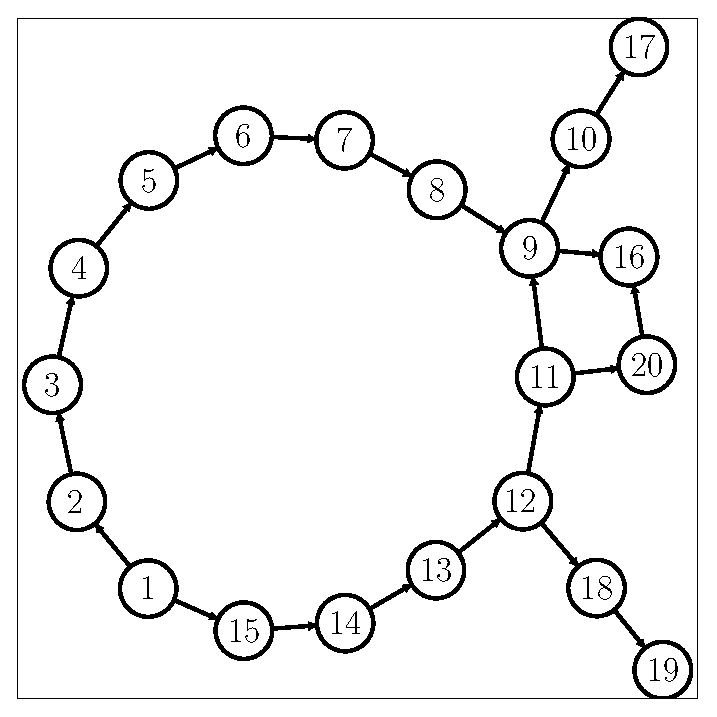
\includegraphics[width=.6\textwidth]{Fig/layout}
  \caption{Layout of test case New York}\label{fig:2}
\end{figure}

For all three programs, namely the hydraulic mixed integer linear program and the reduced hydraulic and thermal linear program, the globally optimal solution is found.
The runtime of the hydraulic mixed integer linear program function \texttt{intlinprog} is about $300\ \si{s}$, while the runtimes of the reduced hydraulic and thermal linear program function \texttt{linprog} are negligible.
These runtime results are obtained with an Intel Core i3-2100 processor.
Furthermore, the runtime result for \texttt{intlinprog} is based on the execution of \texttt{mainNewYork.m}.
However, based on \texttt{mainNewYork.py}, where we access \texttt{intlinprog} through Python wrappers, we obtain a run time of about $600\ \si{s}$.
This is odd since the solution process of the hydraulic mixed integer program with \texttt{intlinprog} conducted through \texttt{mainNewYork.m} and \texttt{mainNewYork.py} only differs in slightly different, but up to machine precision identical, hydraulic data.
Apparently, this slight difference in hydraulic data results in a different \texttt{intlinprog} preprocessing which seems to have a great impact on runtime.
Such an enormous sensitivity is clearly undesirable.

Please note that due to large demands in terms of $\dot{v}_n^{rq}$ and due to a large network in terms of $L_e$, high pressures $p_n$ and high temperatures $T_n^{spp}$, $T_n^{rtn}$ are characteristic for test case New York.

\section{How-To}

\subsection{Port}

In order to run the Matlab main source file \texttt{mainNewYork.m} within a new environment, no adjustments should be required.
Since the Python wrapper implementations interact with Matlab through a UNIX system prompt, running the Python main source file \texttt{mainNewYork.py} on Mac and Linux should be straight forward while running it on Windows might not. 
In order to run the Python main source file \texttt{mainNewYork.py} within a new UNIX environment, the directory name variables \texttt{matlabDir} and \texttt{finalDir} in \texttt{mainNewYork.py} should be adjusted.

\subsection{Run a New Test Case}

A new test case can be defined by providing appropriate replacements of the functions \texttt{setNewYork} in source files \texttt{LayoutData.m} / \texttt{LayoutData.py}, \texttt{HydraulicData.m} / \texttt{HydraulicData.py}, \texttt{ReducedHydraulicData.m} / \texttt{ReducedHydraulicData.py} and \texttt{ThermalData.m} / \texttt{ThermalData.py}.
In order to run the new test case, the main source file \texttt{mainNewYork.m} / \texttt{mainNewYork.py} needs to be changed accordingly.
Please note that the definition of a physically and numerically feasible new test case might be a troublesome process.

\bibliography{reference}
\bibliographystyle{plain}












\end{document}
